\documentclass[12pt]{article}
\usepackage[letterpaper, margin=1in]{geometry}
\usepackage{graphicx}
\usepackage{newtxtext,newtxmath}
\usepackage[hidelinks]{hyperref}
\usepackage{caption}

\pagestyle{empty}
\setlength{\parindent}{0pt}
\setlength{\parskip}{0.4em}

\begin{document}

\begin{center}
{\bfseries Eigenvector Centrality Reveals Structural Undervaluation\\
in U.S. Interstate Commerce Networks}

\vspace{0.3em}
S.\ Thornton\\
Department of Systems Science, Binghamton University
\end{center}

\vspace{0.4em}

GDP counts value produced locally. It says nothing about which states enable production elsewhere. We construct a weighted, directed network of interstate commodity flows (51 nodes, ${\sim}$2,500 edges) from the 2017 Commodity Flow Survey and ask a simple question: which states are structurally important to the national trade system in ways GDP cannot see?

Eigenvector centrality provides a clear answer. The GDP-eigenvector rank correlation is strong (Spearman $\rho = 0.934$), but 39\% of states diverge by five or more positions. Kentucky, for instance, ranks 28th in GDP but 14th in eigenvector centrality. Its commodity flows sustain production in wealthier states, yet this structural role is invisible in output-based accounting. Seven other physical-economy states show similar gains.

This is not merely an academic reranking. Seven of the eight overperformers are now attracting over \$170 billion in AI data center investment (2024--2026). These states share characteristics that also attract compute infrastructure: cheap power, water access, grid capacity, and logistics corridors. A framework applied to 2017 trade data appears to identify structural assets the market has only recently begun to price.

We test boundary sensitivity by comparing the domestic network against a 52-node network including international flows. Eigenvector rankings are robust ($\rho = 0.982$); betweenness centrality is not ($\rho = 0.816$), raising open questions about weight semantics in flow networks.

\vspace{0.3em}
\begin{center}
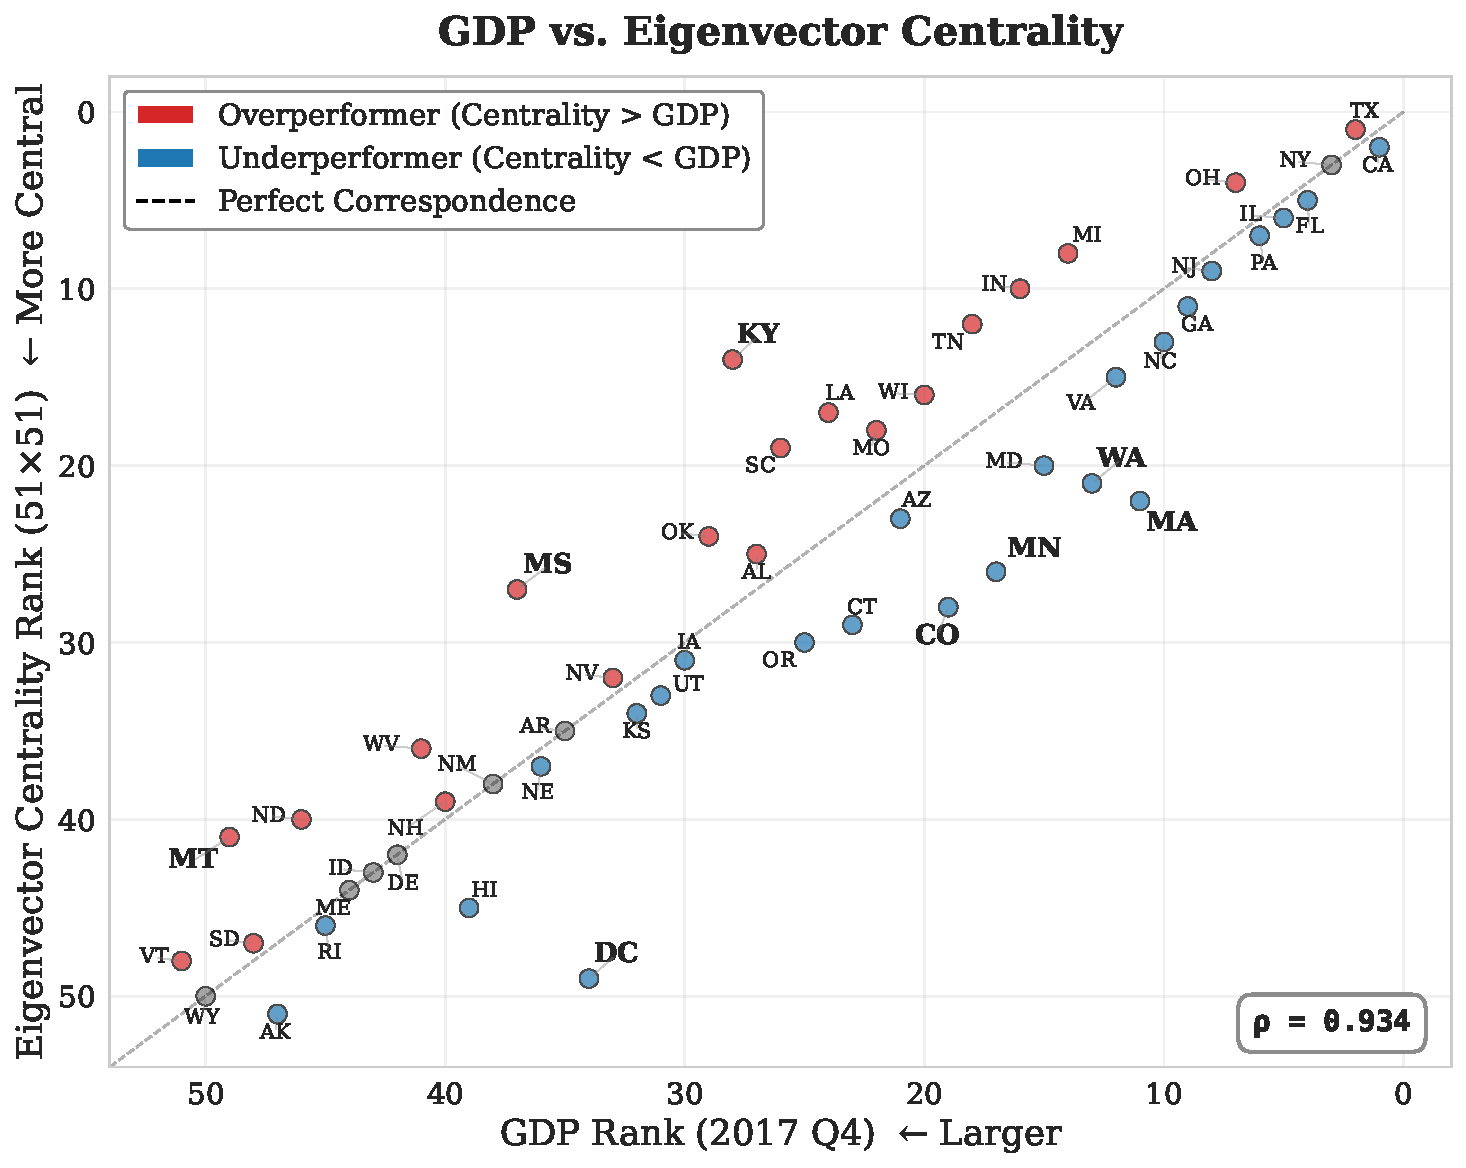
\includegraphics[height=2.8in]{figures/gdp_vs_eigenvector_scatter.pdf}
\captionof{figure}{\small GDP rank vs.\ eigenvector centrality rank for 51 states. States above the diagonal are structurally undervalued by GDP. $\rho = 0.934$.}
\end{center}

\end{document}
